\documentclass[10pt,a4paper]{article}
\usepackage[utf8]{inputenc}
\usepackage{amsmath}
\usepackage{amsfonts}
\usepackage{amssymb}
\usepackage{graphicx}
\begin{document}

\begin{titlepage}

\newcommand{\HRule}{\rule{\linewidth}{0.5mm}} % Defines a new command for the horizontal lines, change thickness here

\center % Center everything on the page
 
\textsc{\LARGE KU Leuven}\\[1.5cm] % Name of your university/college
\textsc{\Large Literature study: dashboards}\\[0.5cm] % Major heading such as course name
\textsc{\large Alcatel-Lucent internship}\\[0.5cm] % Minor heading such as course title


\HRule \\[0.4cm]
{ \huge \bfseries Literature study on dashboards}\\[0.4cm]
\HRule \\[1.5cm]
 

\Large \emph{Author:}\\
Helena \textsc{Brekalo}\\[3cm]

{\large \today}\\[3cm] % Date

\vfill % Fill the rest of the page with whitespace

\end{titlepage}

\section{General}
A dashboard is a tool to quickly show information at a glance. Its purpose is to have the "reader" gather information without having to look things up; everything should be clear by having a quick look at the dashboard. At Alcatel-Lucent, they make use of the Jenkins dashboard, but it doesn't comply with the given description: in order to see what builds failed/succeeded, you need to find the build you're looking for and then check its status. It is clear from the -lack of- its use that this way of displaying the information does not suffice, since the TV dashboard is not/barely used but every employer looks up the dashboard on their own PC every once in a while. \\

The purpose of this literature study is to create Jenkins awareness, so the developers can take a look at the TV dashboard a few times a day and have them see how the project is proceeding.\\
One of the most important things is that the information displayed on the dashboard can be easily interpreted. This means that you don't want a cluttered dashboard with too much information so it becomes unclear.
Stephen Few has written an excellent article on the topic, with the main conclusions being:
\begin{itemize}
\item don't show too much information,
\item keep the information simple,
\item colors should be used sparingly or they will mean nothing at all,
\item visuals should be useful; not overwhelming or distracting and
\item the information represented should be accurate, so you should make sure the information is displayed correctly and with enough context.
\end{itemize}
 
This last remark is also made by Matthew Skelton\footnote{http://blog.matthewskelton.net/2013/03/11/what-makes-an-effective-build-and-deployment-radiator-screen/}, who shows that if you only show the failed builds, people will start to ignore the 'alarm signals' the dashboard displays and perform less well compared to when a context is shown, also showing the successful builds. \\
Few’s theory is backed up by the people at Geckoboard, who have made a blog consisting of 6 parts, referencing to Few, but also adding some rules of thumb\footnote{https://www.geckoboard.com/blog/building-great-dashboards-6-golden-rules-to-successful-dashboard-design/}. Every article listed in the appendix refers to Few’s article and some make additional remarks. 
One of them is that it’s very important to keep your audience in mind, the board of directors will want to see different metrics represented in the dashboard than, say, the people of human resources. 
In the case of software developers, they’ll want to see metrics about the build status of the different jobs. Related to this is that not every dashboard will need the same layout and look. \\
In the case of the Jenkins dashboard, charts won’t tell you much, since it doesn’t really tell anything about the status of the last build. Below, the example of the Jenkins dashboard is further explained and a proposal is made that conforms to the guidelines of a good dashboard.

\section{Improving the Jenkins dashboard}
The Jenkins dashboard, as seen in Figure \ref{jenkins}, displays a list of the builds of a project, together with a colored dot and a "weather report". The dot displays information about the last build, the color indicating whether it failed or succeeded and a flashing dot meaning the build is still in progress. 
The color of the dot at that time then refers to the last finished build.
The weather report tells you something about the stability of the builds. If the weather looks good, then the build is stable. The worse the weather gets, the less stable the build is. This way, you get an overall view about the stability of the different build jobs.

\begin{figure}[ht!]
\centering
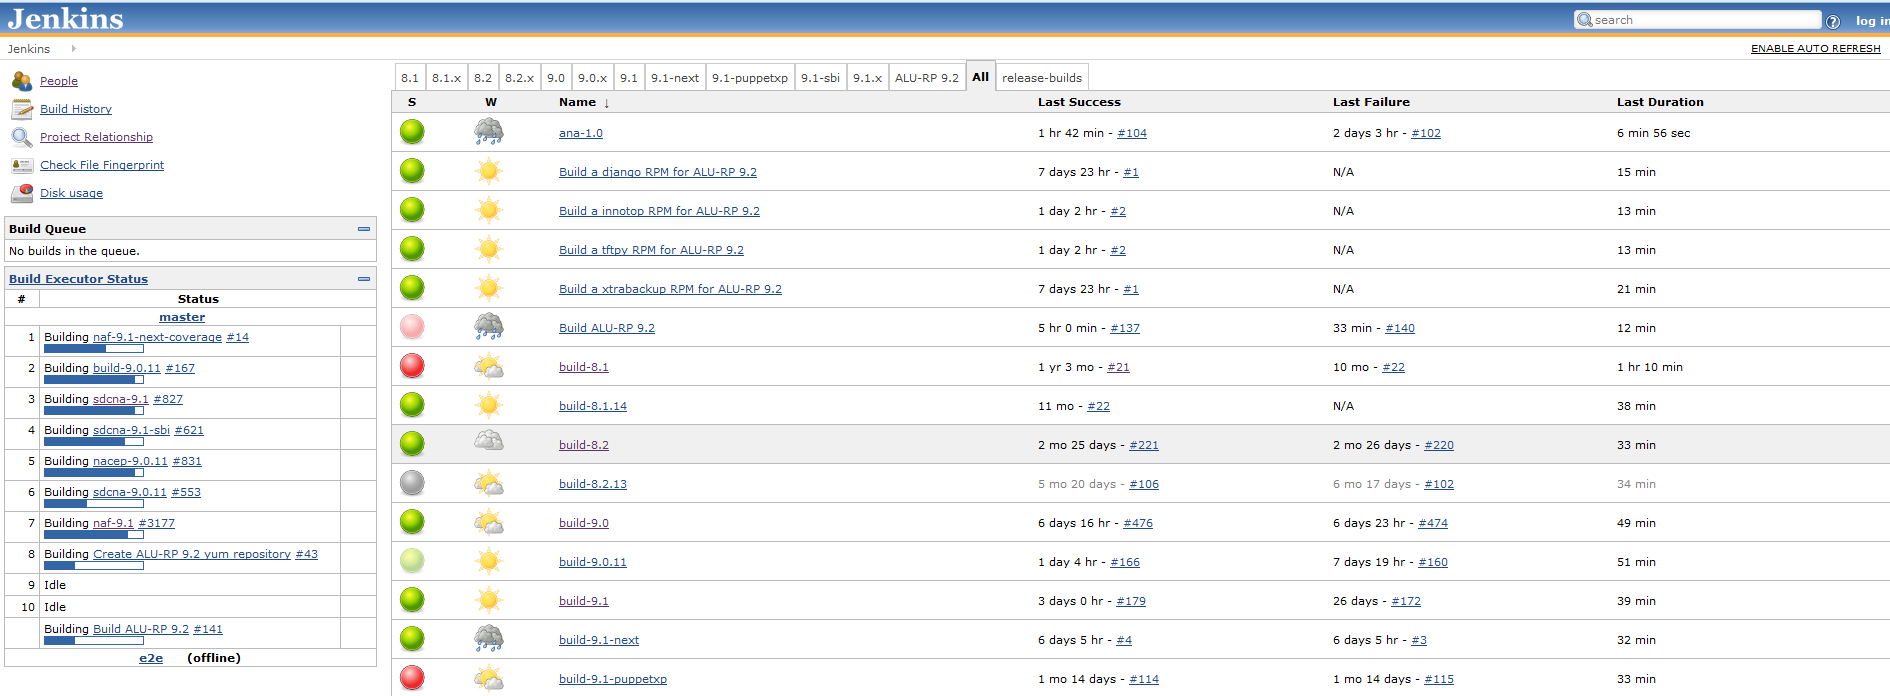
\includegraphics[width=90mm]{CaptureJenkins.png}
\caption{The Jenkins dashboard.} 
\label{jenkins}
\end{figure}
 
These two things give you a fairly good overview, but the downside of the dashboard is that you have to be right in front of the screen to see what job the colored dot and the weather report are referring to. 
The details of the build job are in plain text, so if you want to project it on a TV screen, people will have a hard time knowing what builds are doing well and which ones aren't.
There are plug-ins available that show a dashboard, but they none of them comply with the most important rules described above: they're either too crowded or use too much color, distracting the viewer from what's really important.

\begin{figure}
\centering
\begin{minipage}{0.45\textwidth}
\centering
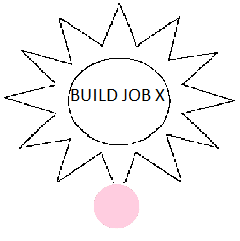
\includegraphics[width=60mm]{prop1.png}
\caption{Proposal 1.}
\label{prop1}
\end{minipage}\hfill
\begin{minipage}{0.45\textwidth}
\centering
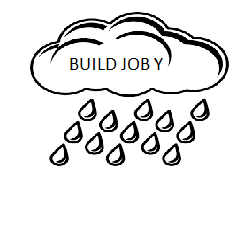
\includegraphics[width=60mm]{prop2.png}
\caption{Proposal 2.}
\label{prop2}
\end{minipage}
\end{figure}
  
The proposed images, as seen in Figure \ref{prop1} and \ref{prop2} comply with the design problems to be avoided as proposed by Stephen Few:
\begin{itemize}
\item Too much complexity
\item Too many alert conditions
\item Alerts that cannot be differentiated
\item Overwhelming visuals
\item Distracting visuals
\item Inappropriate visual salience
\item Mismatch between information and its visual representation
\item Indirect expression of measures
\item Not enough context
\end{itemize}
The images show the build stability together with the success or failure of the last build and show the name of the build clearly. It's also possible to add a timestamp of when the last success and failure were and the last duration at the bottom of the tiles, as shown in Figure \ref{prop2}. If you have color blind people in your team (as Few pointed out might happen), you could replace the green dot by a very light red dot, indicating it doesn't need attention, as shown in Figure \ref{prop1}.
This could be realized using existing Jenkins plug-ins and changing them. The Radiator View\footnote{http://blog.matthewskelton.net/2013/03/11/what-makes-an-effective-build-and-deployment-radiator-screen/} seems like a good basis.
An alternative could be to implement already existing software like Dashing\footnote{dashing.io}, which provides the tools to generate dashboards very easily. Instead of showing the weather as proposed, color codes may be used for the tile backgrounds, either representing the status of the last build or the status of the past builds. A combination is also possible where the color represents the status of the last build and an opaque weather report image as the background. An example is given in Figure \ref{dash}:

\begin{figure}[ht!]
\centering
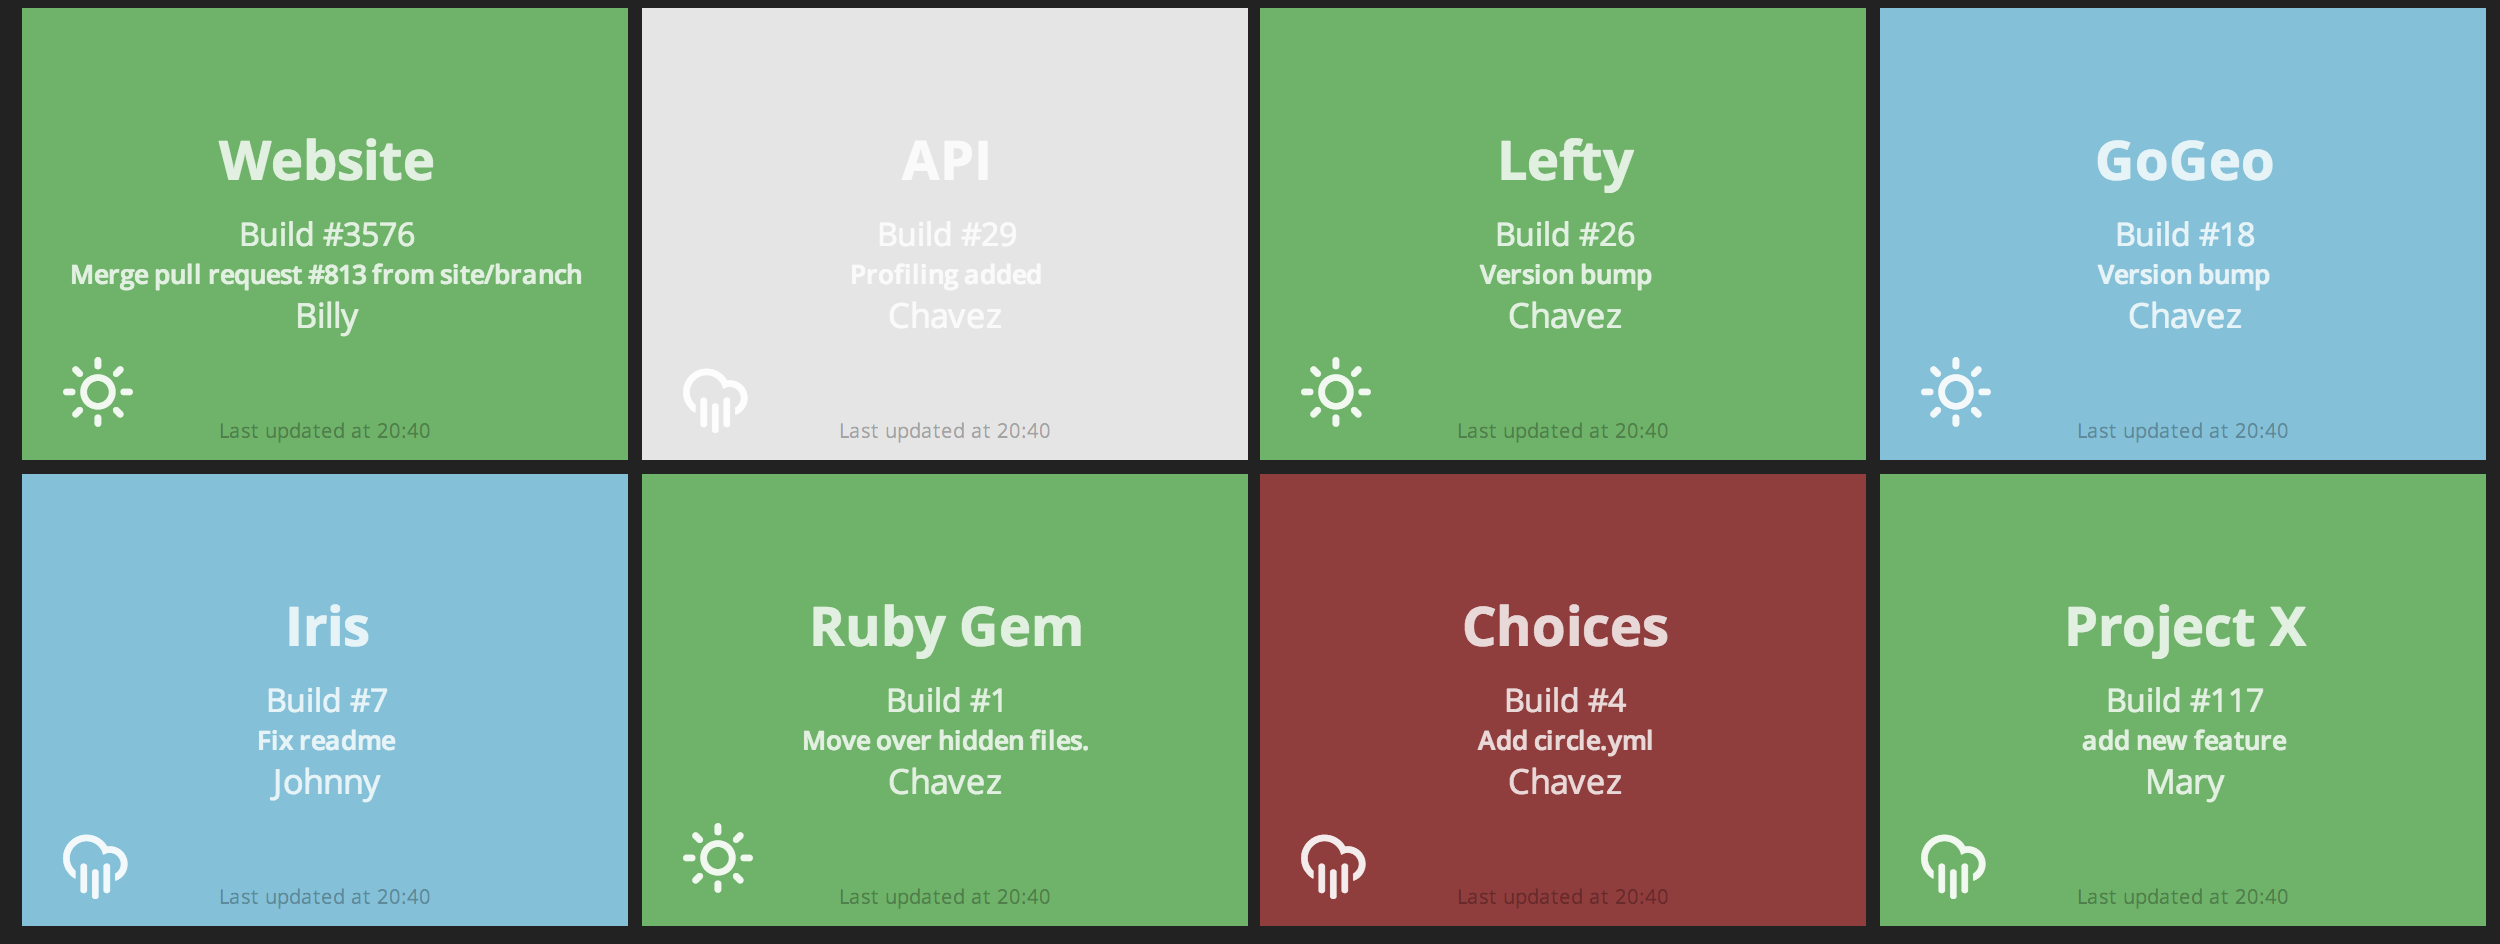
\includegraphics[width=90mm]{dashboard-prop.png}
\caption{Example dashboard for Jenkins.} 
\label{dash}
\end{figure} 
 
The colors aren’t too overwhelming and they’re meaningful, since people are used to the colored dots in the Jenkins dashboard. 
A third, less tile-oriented dashboard is Team Dashboard\footnote{http://fdietz.github.io/team\_dashboard/}. It also supports Jenkins plug-ins.

\clearpage

\begin{thebibliography}{11} 

\bibitem{few} Stephen Few, \emph{Dashboard Design For Real-Time Situation Awareness}, http://www.perceptualedge.com/articles/Whitepapers/Dashboard\_Design.pdf, consulted on 09/07/2015

\bibitem{skelton} Matthew Skelton, \emph{What Makes an Effective Build and Deployment Radiator Screen?}, http://blog.matthewskelton.net/2013/03/11/what-makes-an-effective-build-and-deployment-radiator-screen/, consulted on 09/07/2015

\bibitem{smith} Nick Smith, \emph{Designing and Building Great Dashboards - 6 Golden Rules to Successful Dashboard Design}, https://www.geckoboard.com/blog/building-great-dashboards-6-golden-rules-to-successful-dashboard-design/, consulted on 09/07/2015

\bibitem{gemignani} Zach Gemignani, \emph{A Dashboard Alerts Checklist}, http://www.juiceanalytics.com/writing/dashboard-alerts-checklist/, consulted on 09/07/2015

\bibitem{juice} No author specified, \emph{A Guide to Creating Dashboards People Love to Use}, http://www.cpoc.org/assets/Data/guide\_to\_dashboard\_design1.pdf, consulted on 10/07/2015

Images:

\bibitem{sun} \emph{Sun}, http://azcoloring.com/coloring-page/112445

\bibitem{rain} \emph{Rain cloud}, http://www.clipartpanda.com/categories/animated-rain-clouds

\bibitem{red_dot} \emph{Red dot}, http://www.thepointless.com/reddot

\bibitem{pink_dot} \emph{Pink dot}, http://www.create-a-mural.com/dry-erase-11-soft-pink-dot-decal.html

\bibitem{dashboard} \emph{Example dashboard},  https://camo.githubusercontent.com/
1509a366bd27fad24ba09c45793308a85bcbf8bf/687474703a2f2f662e636c2e6c792f6974656d732
f336330743076335a31313145306f3436333033322f53637265656e25323053686f742532303230313
32d31302d30332532306174253230382e34362e3437253230504d2e706e67

\end{thebibliography}


\end{document}